\documentclass{article}\usepackage[]{graphicx}\usepackage[]{color}
%% maxwidth is the original width if it is less than linewidth
%% otherwise use linewidth (to make sure the graphics do not exceed the margin)
\makeatletter
\def\maxwidth{ %
  \ifdim\Gin@nat@width>\linewidth
    \linewidth
  \else
    \Gin@nat@width
  \fi
}
\makeatother

\definecolor{fgcolor}{rgb}{0.345, 0.345, 0.345}
\newcommand{\hlnum}[1]{\textcolor[rgb]{0.686,0.059,0.569}{#1}}%
\newcommand{\hlstr}[1]{\textcolor[rgb]{0.192,0.494,0.8}{#1}}%
\newcommand{\hlcom}[1]{\textcolor[rgb]{0.678,0.584,0.686}{\textit{#1}}}%
\newcommand{\hlopt}[1]{\textcolor[rgb]{0,0,0}{#1}}%
\newcommand{\hlstd}[1]{\textcolor[rgb]{0.345,0.345,0.345}{#1}}%
\newcommand{\hlkwa}[1]{\textcolor[rgb]{0.161,0.373,0.58}{\textbf{#1}}}%
\newcommand{\hlkwb}[1]{\textcolor[rgb]{0.69,0.353,0.396}{#1}}%
\newcommand{\hlkwc}[1]{\textcolor[rgb]{0.333,0.667,0.333}{#1}}%
\newcommand{\hlkwd}[1]{\textcolor[rgb]{0.737,0.353,0.396}{\textbf{#1}}}%
\let\hlipl\hlkwb

\usepackage{framed}
\makeatletter
\newenvironment{kframe}{%
 \def\at@end@of@kframe{}%
 \ifinner\ifhmode%
  \def\at@end@of@kframe{\end{minipage}}%
  \begin{minipage}{\columnwidth}%
 \fi\fi%
 \def\FrameCommand##1{\hskip\@totalleftmargin \hskip-\fboxsep
 \colorbox{shadecolor}{##1}\hskip-\fboxsep
     % There is no \\@totalrightmargin, so:
     \hskip-\linewidth \hskip-\@totalleftmargin \hskip\columnwidth}%
 \MakeFramed {\advance\hsize-\width
   \@totalleftmargin\z@ \linewidth\hsize
   \@setminipage}}%
 {\par\unskip\endMakeFramed%
 \at@end@of@kframe}
\makeatother

\definecolor{shadecolor}{rgb}{.97, .97, .97}
\definecolor{messagecolor}{rgb}{0, 0, 0}
\definecolor{warningcolor}{rgb}{1, 0, 1}
\definecolor{errorcolor}{rgb}{1, 0, 0}
\newenvironment{knitrout}{}{} % an empty environment to be redefined in TeX

\usepackage{alltt}
\usepackage{amsmath}
\IfFileExists{upquote.sty}{\usepackage{upquote}}{}
\begin{document}
%\SweaveOpts{concordance=TRUE}

\begin{knitrout}
\definecolor{shadecolor}{rgb}{0.969, 0.969, 0.969}\color{fgcolor}\begin{kframe}


{\ttfamily\noindent\itshape\color{messagecolor}{\#\# Registering fonts with R}}

{\ttfamily\noindent\color{warningcolor}{\#\# Warning: package 'ggplot2' was built under R version 3.3.3}}

{\ttfamily\noindent\color{warningcolor}{\#\# Warning: package 'xtable' was built under R version 3.3.3}}\end{kframe}
\end{knitrout}


\section{Description}
The symetric random walk will be described in this document (Mt). it covers the theory of "Stochastic Calculus for finance" Tome 2 chapter 3 section 1.

The construction of the random walk depend on the evolution of a random variable $X_i$. The previous RV can take two value at each time, like tossing a coin. $X_i$ can take the value 1 or -1.

\begin{equation}
 \label{eq:Xi}
X_i = 
\left \{{
  \begin{array}{c} 1 \\ -1 \end{array}
  }\right .
\end{equation}
 
The Symetric Random Walk is constructed by summing up the different outcome of the random variable $X_i$ from $k$ experiments:

\begin{equation}
\label{eq:SRW}
M_k = 
\sum_{j=1}^k X_j
\end{equation}

In the following lines of code, $X_i$ is randomly difined. The variable $k$ ensure to have a sufficent number of periods to further generate the scaled random walk.
It refers to the $k$ of equation~\ref{eq:SRW}.
$p$ and $q$ are the probability measure, respectively $p$ chance to get value 1 and $q$ chance to get -1 from random variable $X_i$.

 


After creating the random variable $X_i$ it suffices to add up all the differente output we get from time 1 up to $k$ to get a specific Symetric Random Walk.

The following outcome present a randomly generated 300 steps symmetric random walk.

\begin{table}[h]

\caption{300 steps Symmetric Random Walk}
\end{table}


\begin{figure}[!h]
\begin{center}

\begin{knitrout}
\definecolor{shadecolor}{rgb}{0.969, 0.969, 0.969}\color{fgcolor}
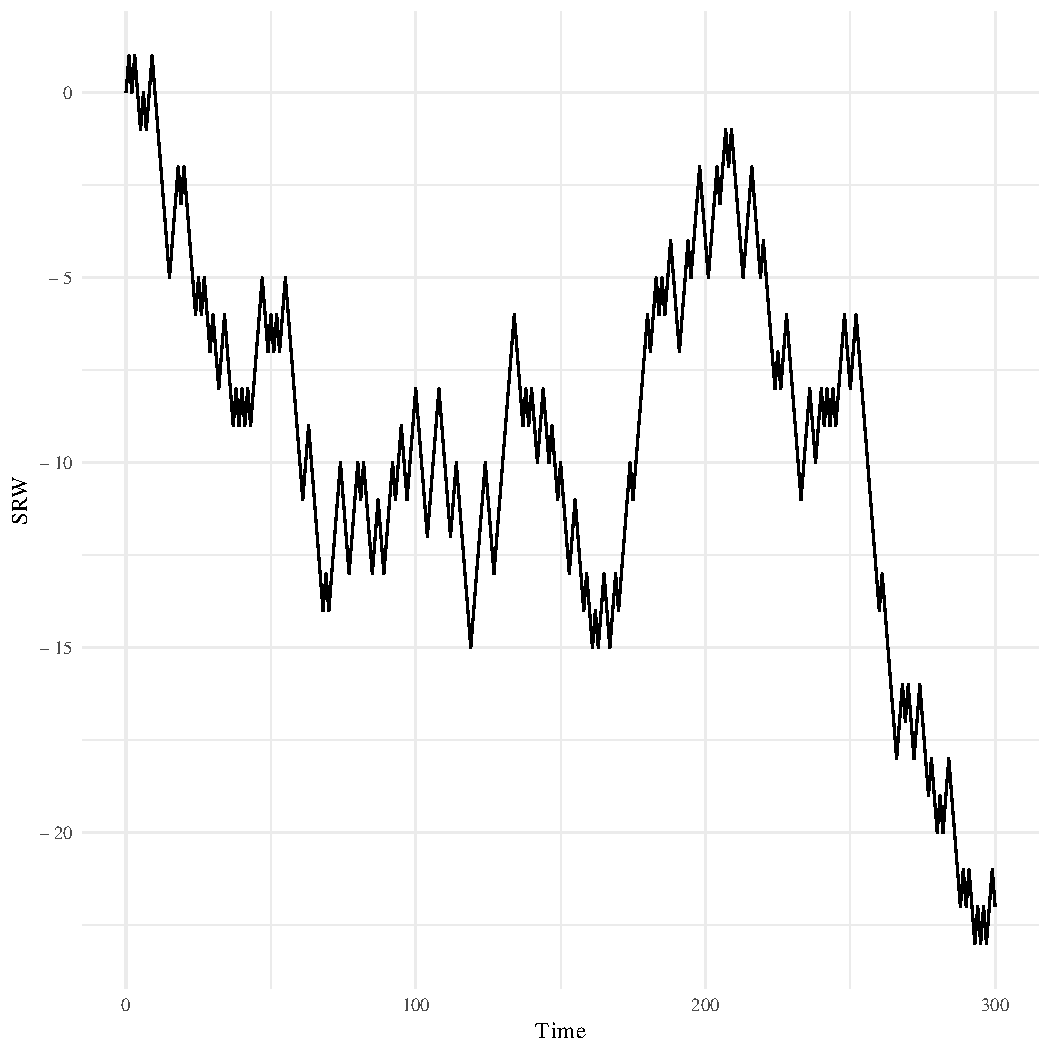
\includegraphics[width=1\linewidth]{figure/unnamed-chunk-4-1} 

\end{knitrout}


\end{center}
\caption{Symmetric Random Walk}
\end{figure}

\begin{kframe}
\begin{alltt}
\hlstd{Mk} \hlkwb{<-} \hlstd{fi} \hlkwb{<-} \hlkwd{data.frame}\hlstd{(}\hlkwd{matrix}\hlstd{(}\hlkwd{rep}\hlstd{(}\hlnum{0}\hlstd{, (k} \hlopt{+} \hlnum{1}\hlstd{)}\hlopt{^}\hlnum{2}\hlstd{),} \hlkwc{nrow} \hlstd{= k} \hlopt{+} \hlnum{1}\hlstd{))}
\hlkwa{for}\hlstd{(j} \hlkwa{in} \hlnum{1}\hlopt{:}\hlstd{(k} \hlopt{+} \hlnum{1}\hlstd{))}
 \hlkwa{for}\hlstd{(i} \hlkwa{in} \hlnum{1}\hlopt{:}\hlstd{j)}
   \hlstd{Mk[i,j]} \hlkwb{<-} \hlstd{(j}\hlopt{-}\hlstd{i)} \hlopt{+} \hlstd{(}\hlnum{1}\hlopt{-}\hlstd{i)}
\hlkwd{xtable}\hlstd{(Mk[}\hlnum{1}\hlopt{:}\hlnum{10}\hlstd{,} \hlnum{1}\hlopt{:}\hlnum{10}\hlstd{])}
\end{alltt}
\end{kframe}% latex table generated in R 3.3.2 by xtable 1.8-2 package
% Fri May 12 15:43:43 2017
\begin{table}[ht]
\centering
\begin{tabular}{rrrrrrrrrrr}
  \hline
 & X1 & X2 & X3 & X4 & X5 & X6 & X7 & X8 & X9 & X10 \\ 
  \hline
1 & 0.00 & 1.00 & 2.00 & 3.00 & 4.00 & 5.00 & 6.00 & 7.00 & 8.00 & 9.00 \\ 
  2 & 0.00 & -1.00 & 0.00 & 1.00 & 2.00 & 3.00 & 4.00 & 5.00 & 6.00 & 7.00 \\ 
  3 & 0.00 & 0.00 & -2.00 & -1.00 & 0.00 & 1.00 & 2.00 & 3.00 & 4.00 & 5.00 \\ 
  4 & 0.00 & 0.00 & 0.00 & -3.00 & -2.00 & -1.00 & 0.00 & 1.00 & 2.00 & 3.00 \\ 
  5 & 0.00 & 0.00 & 0.00 & 0.00 & -4.00 & -3.00 & -2.00 & -1.00 & 0.00 & 1.00 \\ 
  6 & 0.00 & 0.00 & 0.00 & 0.00 & 0.00 & -5.00 & -4.00 & -3.00 & -2.00 & -1.00 \\ 
  7 & 0.00 & 0.00 & 0.00 & 0.00 & 0.00 & 0.00 & -6.00 & -5.00 & -4.00 & -3.00 \\ 
  8 & 0.00 & 0.00 & 0.00 & 0.00 & 0.00 & 0.00 & 0.00 & -7.00 & -6.00 & -5.00 \\ 
  9 & 0.00 & 0.00 & 0.00 & 0.00 & 0.00 & 0.00 & 0.00 & 0.00 & -8.00 & -7.00 \\ 
  10 & 0.00 & 0.00 & 0.00 & 0.00 & 0.00 & 0.00 & 0.00 & 0.00 & 0.00 & -9.00 \\ 
   \hline
\end{tabular}
\end{table}


















\end{document}
